\section{Ingestion module for the REP\_PASS\_E file}

This sections describes the ingestion module for inserting the \acrshort{efep} acquisition analysis after reception of data from the satellite.

The associated ingestion processor is:

\begin{itemize} 

\item \textbf{s2boa.ingestions.ingestion\_edrs\_acquisition.ingestion\_edrs\_acquisition}

\item \textbf{s2boa.ingestions.ingestion\_vgs\_acquisition.ingestion\_vgs\_acquisition}
  
\end{itemize}

This module uses the following \acrshort{dim} signatures:

\begin{itemize} 

\item \textbf{RECEPTION\_XXX}: data corresponding to the acquisition analysis after reception of data from the satellite.

\item \textbf{COMPLETENESS\_NPPF\_XXX}: data corresponding to the definition of planning completeness used for analysis.

\item \textbf{ISP\_VALIDITY\_PROCESSING\_COMPLETENESS\_XXX}: data corresponding to the definition of \acrshort{isp} processing completeness used for analysis.

\end{itemize}

Where XXX is the corresponding satellite id, SSS is the station ID and VVV is the \acrshort{vcid} number.

The figure \ref{fg:structure_ingestion_eisp} shows a simplified diagram of the structure of the data inserted (associated structure of values not included for simplicity).

\begin{figure}[H]
  \begin{center}
	\centering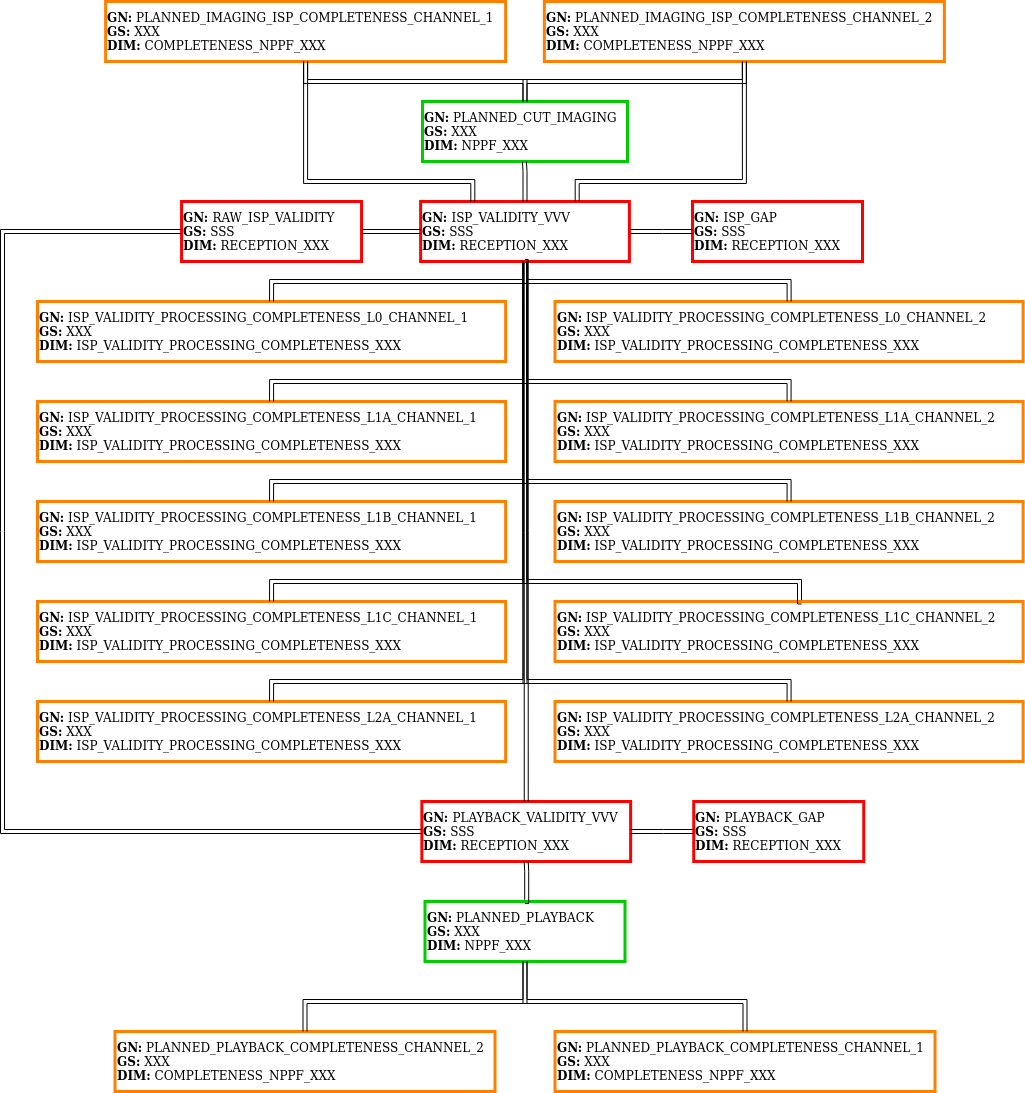
\includegraphics[width=150mm]{../fig/structure_ingestion_eisp.png}
	\caption{Structure of the data inserted by the ingestion module for the REP\_PASS\_[2|5] file}
	\label{fg:structure_ingestion_eisp}
  \end{center}
\end{figure}

The table \ref{tb:description_events_ingestion_eisp} shows the description of the events inserted by the ingestion.

\begin{landscape}
\begin{longtable}{|M{0.15\linewidth}|M{0.05\linewidth}|M{0.15\linewidth}|M{0.2\linewidth}|M{0.15\linewidth}|M{0.15\linewidth}|}
\hline \textbf{Gauge name} & \textbf{Gauge system}  & \textbf{DIM signature} & \textbf{Description} & \textbf{Start} & \textbf{Stop} \\ \hline
\textbf{PLAYBACK\_VALIDITY\_VVV} & SSS & RECEPTION\_XXX & Event for representing the \textbf{ground acquisition operation} & UTC time associated to the start of the reception & UTC time associated to the stop of the reception \\ \hline
\textbf{PLAYBACK\_GAP} & SSS & RECEPTION\_XXX & Event for representing a \textbf{gap in the ground acquisition operation} & UTC time associated to the start of the corresponding gap in the reception & UTC time associated to the stop of the corresponding gap in the reception \\ \hline
\textbf{PLANNED\_PLAYBACK\_COMPLETENESS\_CHANNEL\_1} & XXX & COMPLETENESS\_NPPF\_XXX & Event for completing the \textbf{expectation of the planned playbacks through the channel 1} & Start of the reception through the channel 1 & Stop of the reception through the channel 1 \\ \hline
\textbf{PLANNED\_PLAYBACK\_COMPLETENESS\_CHANNEL\_2} & XXX & COMPLETENESS\_NPPF\_XXX & Event for completing the \textbf{expectation of the planned playbacks through the channel 2} & Start of the reception through the channel 2 & Stop of the reception through the channel 2 \\ \hline
\textbf{PLANNED\_IMAGING\_ISP\_COMPLETENESS\_CHANNEL\_1} & XXX & COMPLETENESS\_NPPF\_XXX & Event for completing the \textbf{expectation of the planned imaging sent through the channel 1} & Start of the first received scene thorugh the channel 1 of the corresponding continuous \acrshort{msi} segment & Stop of the last received scene thorugh the channel 1 of the corresponding continuous \acrshort{msi} segment \\ \hline
\textbf{PLANNED\_IMAGING\_ISP\_COMPLETENESS\_CHANNEL\_2} & XXX & COMPLETENESS\_NPPF\_XXX & Event for completing the \textbf{expectation of the planned imaging sent through the channel 2} & Start of the first received scene thorugh the channel 2 of the corresponding continuous \acrshort{msi} segment & Stop of the last received scene thorugh the channel 2 of the corresponding continuous \acrshort{msi} segment \\ \hline
\textbf{RAW\_ISP\_VALIDITY} & SSS & RECEPTION\_XXX & Event for representing the \textbf{ground acquisition operation} & Start of the first received scene & Stop of the last received scene \\ \hline
\textbf{ISP\_VALIDITY} & SSS & RECEPTION\_XXX & Event for representing the \textbf{ground acquisition operation} & Start of the first received scene of the corresponding continuous \acrshort{msi} segment & Stop of the last received scene of the corresponding continuous \acrshort{msi} segment \\ \hline
\textbf{ISP\_GAP} & SSS & RECEPTION\_XXX & Event for representing a \textbf{gap in the ground acquisition operation} & UTC time associated to the start of the corresponding continuous gap in the received MSI & UTC time associated to the stop of the corresponding continuous gap in the received MSI \\ \hline
\textbf{ISP\_VALIDITY\_PROCESSING\_COMPLETENESS\_L0\_CHANNEL\_1} & XXX & COMPLETENESS\_NPPF\_XXX & Event for representing the \textbf{expectation of the processing of the planned imaging for the L0} & Start of the first received scene of the corresponding continuous \acrshort{msi} segment & Stop of the last received scene of the corresponding continuous \acrshort{msi} segment \\ \hline
\textbf{ISP\_VALIDITY\_PROCESSING\_COMPLETENESS\_L1A\_CHANNEL\_1} & XXX & COMPLETENESS\_NPPF\_XXX & Event for representing the \textbf{expectation of the processing of the planned imaging for the L0} & Start of the first received scene of the corresponding continuous \acrshort{msi} segment & Stop of the last received scene of the corresponding continuous \acrshort{msi} segment \\ \hline
\textbf{ISP\_VALIDITY\_PROCESSING\_COMPLETENESS\_L1B\_CHANNEL\_1} & XXX & COMPLETENESS\_NPPF\_XXX & Event for representing the \textbf{expectation of the processing of the planned imaging for the L0} & Start of the first received scene of the corresponding continuous \acrshort{msi} segment & Stop of the last received scene of the corresponding continuous \acrshort{msi} segment \\ \hline
\textbf{ISP\_VALIDITY\_PROCESSING\_COMPLETENESS\_L1C\_CHANNEL\_1} & XXX & COMPLETENESS\_NPPF\_XXX & Event for representing the \textbf{expectation of the processing of the planned imaging for the L0} & Start of the first received scene of the corresponding continuous \acrshort{msi} segment & Stop of the last received scene of the corresponding continuous \acrshort{msi} segment \\ \hline
\textbf{ISP\_VALIDITY\_PROCESSING\_COMPLETENESS\_L2A\_CHANNEL\_1} & XXX & COMPLETENESS\_NPPF\_XXX & Event for representing the \textbf{expectation of the processing of the planned imaging for the L0} & Start of the first received scene of the corresponding continuous \acrshort{msi} segment & Stop of the last received scene of the corresponding continuous \acrshort{msi} segment \\ \hline
\textbf{ISP\_VALIDITY\_PROCESSING\_COMPLETENESS\_L0\_CHANNEL\_2} & XXX & COMPLETENESS\_NPPF\_XXX & Event for representing the \textbf{expectation of the processing of the planned imaging for the L0} & Start of the first received scene of the corresponding continuous \acrshort{msi} segment & Stop of the last received scene of the corresponding continuous \acrshort{msi} segment \\ \hline
\textbf{ISP\_VALIDITY\_PROCESSING\_COMPLETENESS\_L1A\_CHANNEL\_2} & XXX & COMPLETENESS\_NPPF\_XXX & Event for representing the \textbf{expectation of the processing of the planned imaging for the L0} & Start of the first received scene of the corresponding continuous \acrshort{msi} segment & Stop of the last received scene of the corresponding continuous \acrshort{msi} segment \\ \hline
\textbf{ISP\_VALIDITY\_PROCESSING\_COMPLETENESS\_L1B\_CHANNEL\_2} & XXX & COMPLETENESS\_NPPF\_XXX & Event for representing the \textbf{expectation of the processing of the planned imaging for the L0} & Start of the first received scene of the corresponding continuous \acrshort{msi} segment & Stop of the last received scene of the corresponding continuous \acrshort{msi} segment \\ \hline
\textbf{ISP\_VALIDITY\_PROCESSING\_COMPLETENESS\_L1C\_CHANNEL\_2} & XXX & COMPLETENESS\_NPPF\_XXX & Event for representing the \textbf{expectation of the processing of the planned imaging for the L0} & Start of the first received scene of the corresponding continuous \acrshort{msi} segment & Stop of the last received scene of the corresponding continuous \acrshort{msi} segment \\ \hline
\textbf{ISP\_VALIDITY\_PROCESSING\_COMPLETENESS\_L2A\_CHANNEL\_2} & XXX & COMPLETENESS\_NPPF\_XXX & Event for representing the \textbf{expectation of the processing of the planned imaging for the L0} & Start of the first received scene of the corresponding continuous \acrshort{msi} segment & Stop of the last received scene of the corresponding continuous \acrshort{msi} segment \\ \hline
\caption{Table describing the events associated to the ingestion}
\label{tb:description_events_ingestion_eisp}
\end{longtable}
\end{landscape}
